\section*{Threat Evaluation}
\addcontentsline{toc}{section}{Threat Evaluation}

Following the identification of the supporting asset, a set of threats and related vulnerabilities were described. 

As shown in figure \ref{fig:threatsEval}, the threats with the highest impacts are the ones tied to the private network and the virtual desktop infrastructure. In particular, those threats are unauthorized wired connections and hyperjacking\cite{online:hyperjacking}. 

These threats were chosen assuming poor access control on the routing equipment of the network and by searching for disrupting incidents for hypervisors. 

Another class belongs to the physical realm. More specifically, the threats tied to the physical access to the server rooms and the natural incidents to which the appliances can be exposed were taken into consideration. As can be seen in the table, the impact of these threats is high and cannot be left untreated.

Finally, only the two threats tied to the \texttt{GSB LAN gateway} were found to have attenuating circumstances. This is because we are considering the gateway of a single municipality, so the incidents will be limited to that GSB.\\

\noindent \textcolor{blue}{Update:} following the descriptions of the studied CVEs and related threat scenarios. 

\subsection*{Session Hijacking - CVE-2021-22927}

This vulnerability affects Citrix Application Delivery Controller (Citrix ADC). An application delivery controller, among its other functions, is responsible for applying security policies. In particular, the infrastructure uses a third-party provider for authentication, entailing the fact that the ADC is configured as a SAML service provider (pre-condition for exploiting the vulnerability).

\subsubsection*{Threat scenario}

To carry out the session fixation attack, an adversary can connect to the application served by the ADC in order to be assigned with a saml-session id. Since the vulnerability states that no privilege are required, we assume that the ADC will assign the id without the need of authentication.

Once the attacker has retrieved the valid id, he/she will need to convince the victim to open a session with the application using the known session id. In the case of a web application, this can be done by convincing a user to open a link in the form of \\ \texttt{https://some.cool.application.com/?SID=SERVER\_SET\_ID\_123456789}.

When the victim performs a login, the adversary will hijack the session using the known session id.\cite{article:kolsek2002session} Now, the attacker has the privileges of the legitimate user.

\subsubsection*{Notes on likelihood}

Exploiting the vulnerability as in the threat scenario have an high risk of detection and punishment since an attacker needs to employ some social engineering on the victim and probably just an e-mail wouldn't suffice.

Furthermore, the amount of required skills to employ successful social engineering practices is not underestimated.

\subsection*{Reverse Shell Attack - CVE-2022-38652}

This vulnerability consists in an insecure deserialization, also called object injection. It affects the software agent of VMWare Hyperic suite, version 5.8.6. In particular, the affected CPE is \\ \href{https://nvd.nist.gov/products/cpe/detail/5976A94C-7191-4547-8205-494B8379A0A3?namingFormat=2.3&orderBy=CPEURI&keyword=cpe%3A2.3%3Aa%3Avmware%3Ahyperic_agent%3A5.8.6%3A*%3A*%3A*%3A*%3A*%3A*%3A*&status=FINAL%2CDEPRECATED}{\texttt{cpe:2.3:a:vmware:hyperic\_agent:5.8.6:*:*:*:*:*:*:*}}.\\

For the following threat scenario description, we assume that the vulnerable software runs on the host operating system of the municipality PC.

\subsubsection*{Threat scenario}

As stated in the NVD database\cite{online:cve-2022-38652}, to leverage the vulnerability, some not specified authentication material is needed from the VMWare Hyperic Server. To obtain that, the exploit of CVE-2022-38650 is required.

Note that the vulnerabilities afflicting the server and the software agent are of the same type\cite{online:cve-2022-38650}. We assume similar threat scenarios exploiting the two vulnerabilities.

To leverage the vulnerability, an adversary can craft a serialized object \texttt{so} starting from a byte stream \texttt{bs} controlled by him/her. Subsequently, the attacker sends \texttt{so} to the victim that will deserialize it, obtaining \texttt{bs}. The deserialized object can contain a call to a function used to run arbitrary code with the privilege of the calling process\cite{artile:Java_Deserialization_Remote-Code_Execution}. For example, in Java such method can be \texttt{Runtime.exec()}.

Since this process is often running with \texttt{SYSTEM} privileges\cite{online:cve-2022-38652}, also the malicious code will inherit \texttt{SYSTEM} privileges. At this point an adversary can open an SSH session on any port he/she prefers. As a result, the attacker has completely violated the host machine, granting him/her the power of manipulating the election inputted data.

\subsubsection*{Notes on likelihood}

Even if this vulnerability requires an attacker to follow an attack chain (through CVE-2022-38650 and 38652), the exploit of these two vulnerabilities is assumed to be fairly similar and not too complex (see also the base metrics). Nonetheless, the means required to execute the attack, the "authentication material" need to be exfiltrated from the server.

\begin{figure}[h!]
    \centering
    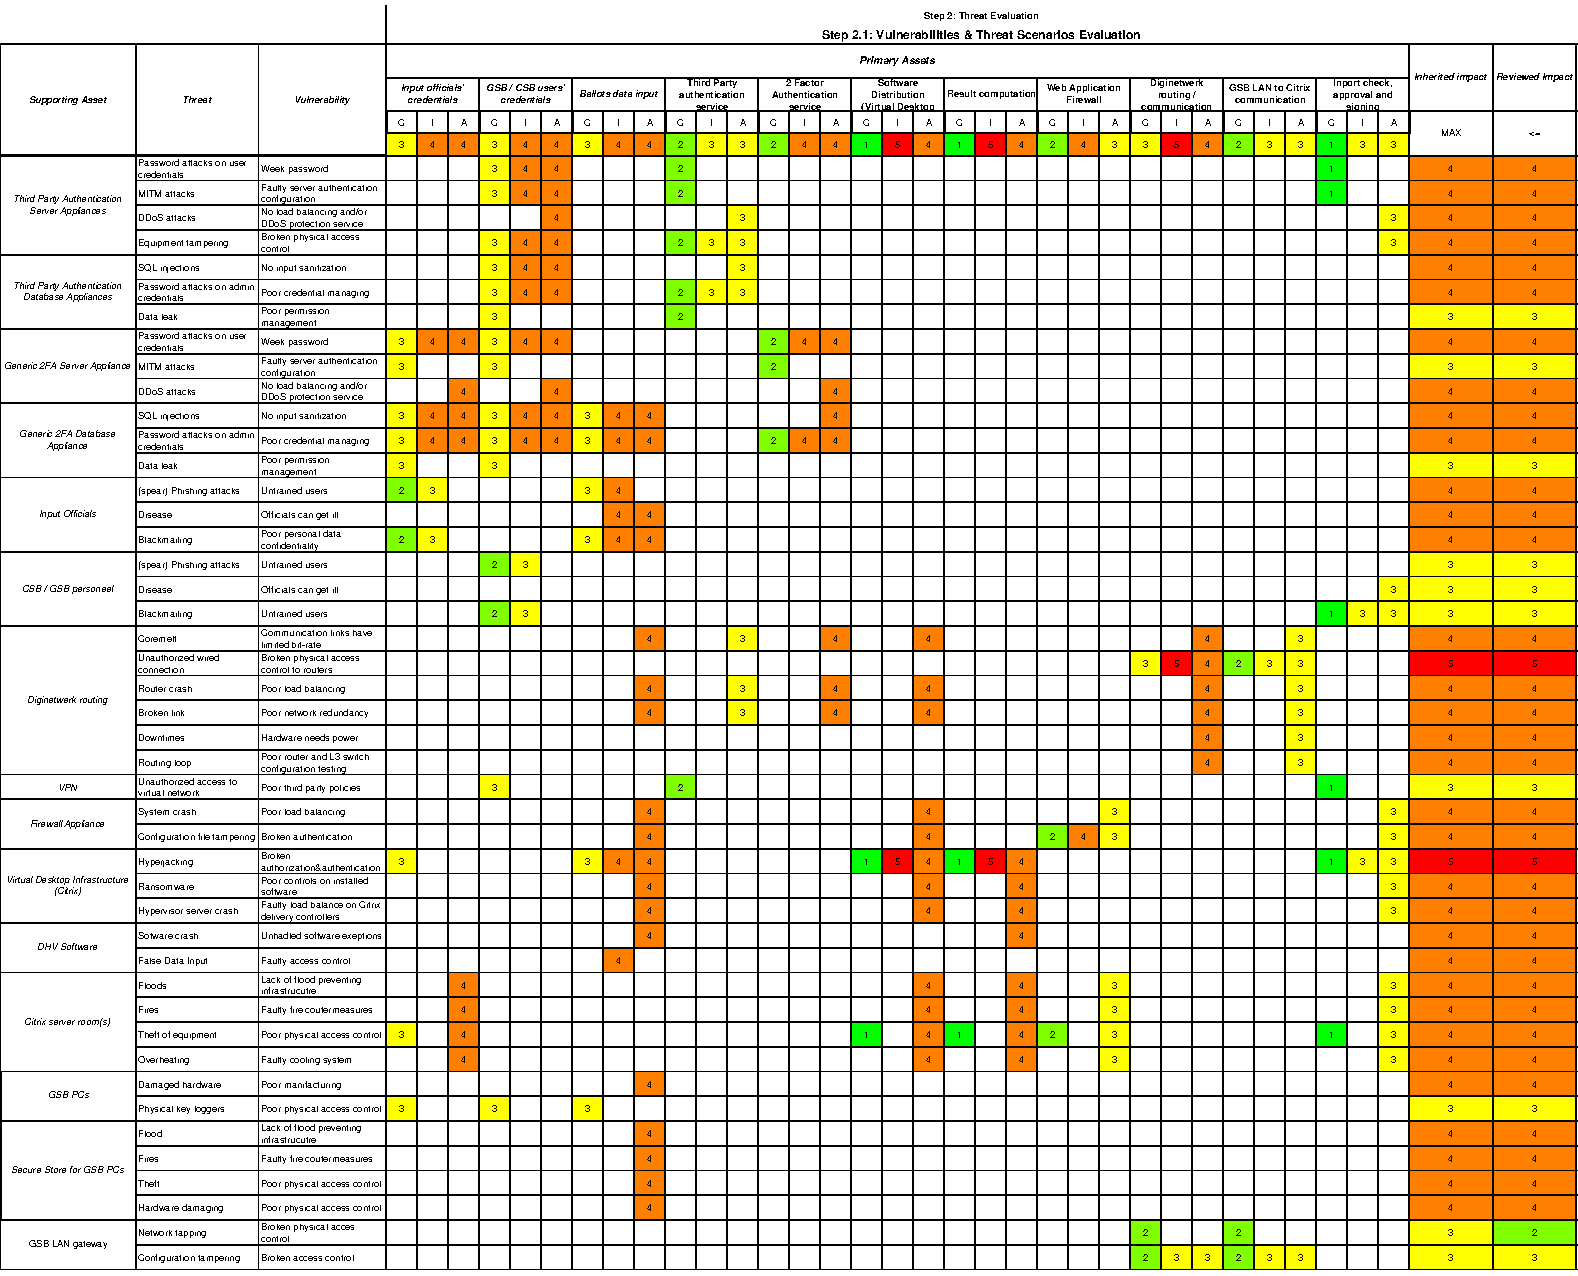
\includegraphics[keepaspectratio,width=1\textwidth]{03-risk-analysis/003-TE/img/threatEval.pdf}
    \caption{Threat evaluation table}
    \label{fig:threatsEval}
\end{figure}

\newpage

Figure \ref{fig:likelihood} shows how likely it is for an incident tied to a threat to happen. For accidental incidents and natural disasters, only the overall score is assigned.

As can be seen in the table, the majority of the threats with higher impacts like Coremelt are mitigated by their low likelihood. Unfortunately, threats like hyperjacking, equipment theft, and tampering still retain a high likelihood score.

Also, historical events were taken into consideration. In particular, since this system is deployed in the Netherlands, data about flooding was researched\cite{online:flooding}.

Note that justifications for the likelihood table can be found in the excel file.

\begin{figure}[]
    \centering
    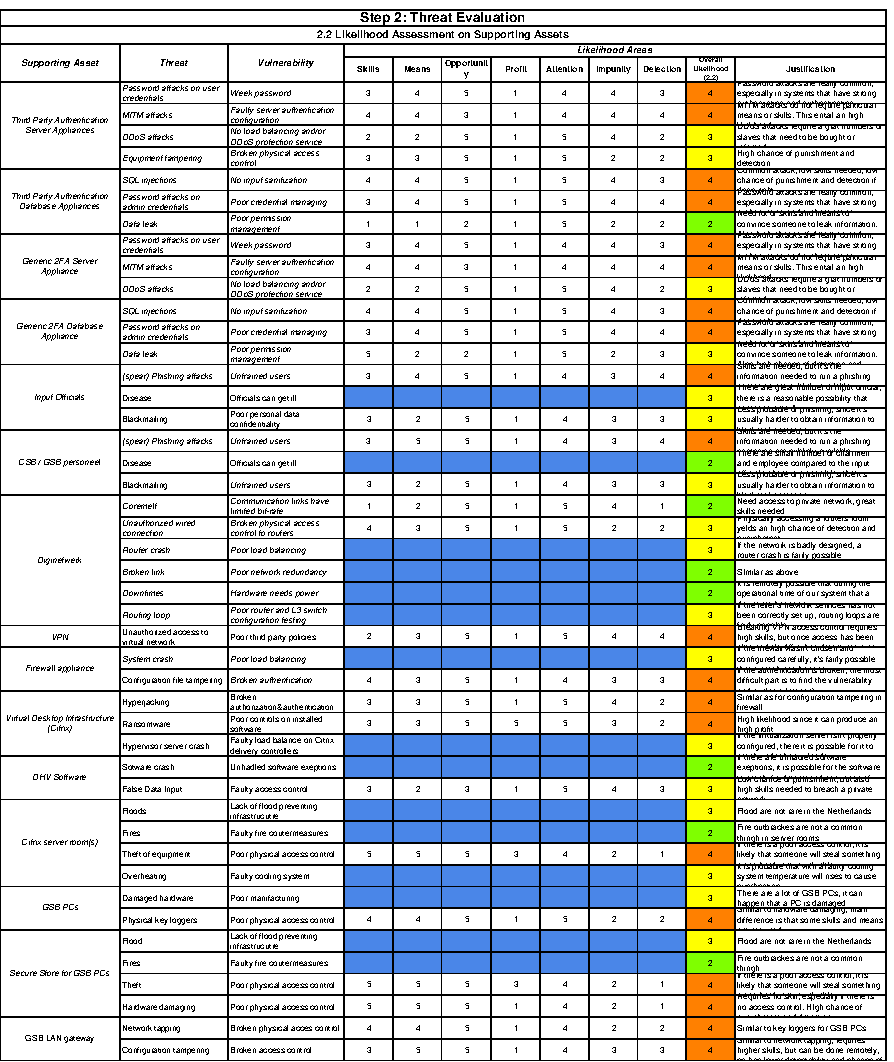
\includegraphics[keepaspectratio,width=1\textwidth]{03-risk-analysis/003-TE/img/likelihood.pdf}
    \caption{Threat likelihood table}
    \label{fig:likelihood}
\end{figure}